%%%%%%%%%%%%%%%%%%%%%%%%%%%%%%%%%%%%%%%%%%%%%%%%%%%%%%%%%%%%%%%%%%%%%%%%%%%%%
%
% annie.tex
%
% hamish, 25/8/1
%
% $Id: annie.tex,v 1.35 2005/11/25 13:23:43 diana Exp $
%
%%%%%%%%%%%%%%%%%%%%%%%%%%%%%%%%%%%%%%%%%%%%%%%%%%%%%%%%%%%%%%%%%%%%%%%%%%%%%


%%%%%%%%%%%%%%%%%%%%%%%%%%%%%%%%%%%%%%%%%%%%%%%%%%%%%%%%%%%%%%%%%%%%%%%%%%%%%
\chapt[chap:annie]{ANNIE: a Nearly-New Information Extraction System}
\markboth{ANNIE: a Nearly-New Information Extraction System}{ANNIE: a Nearly-New Information Extraction System}
%%%%%%%%%%%%%%%%%%%%%%%%%%%%%%%%%%%%%%%%%%%%%%%%%%%%%%%%%%%%%%%%%%%%%%%%%%%%%
\nnormalsize
%%%% qqqqqqqqqqqqqqqqqqqqqqqqq %%%%
\ifprintedbook 
\else
\begin{quote}
And so the time had passed predictably and soberly enough
in work and routine chores, and the events of the previous night from
first to last had faded; and only now that
both their days' work was over, the child asleep and
no further disturbance anticipated, did
the shadowy figures from the masked ball, the melancholy
stranger and the dominoes in red, revive; and those trivial encounters
became magically and painfully interfused with the treacherous illusion
of missed opportunities. Innocent yet ominous questions and
vague ambiguous answers passed to and fro between them; and,
as neither of them doubted the other's absolute candour, both felt
the need for mild revenge. They exaggerated the extent to which their
masked partners had attracted them, made fun of the jealous
stirrings the other revealed, and lied dismissively about their own.
Yet this light banter about the trivial adventures of the previous
night led to more serious discussion of those hidden, scarcely
admitted desires which are apt to raise dark and perilous storms even
in the purest, most transparent soul; and they talked about those secret
regions for which they felt hardly any longing, yet towards
which the irrational wings of fate might one day drive them, if
only in their dreams. For however much they might belong to one
another heart and soul, they knew last night was not the first
time they had been stirred by a whiff of freedom, danger and adventure.

{\it Dream Story}, Arthur Schnitzler, 1926 (pp. 4-5).
\end{quote}
\fi
%%%% qqqqqqqqqqqqqqqqqqqqqqqqq %%%%


GATE was originally developed in the context of
\htlink{http://gate.ac.uk/ie/}{Information Extraction}
(IE) R\&D, and IE systems in many languages and shapes and sizes have
been created using GATE with the IE components that have been
distributed with it (see \cite{May00a} for descriptions of some of
these projects).\footnote{The principal architects of the IE systems
in GATE version 1 were
\htlink{http://www.dcs.shef.ac.uk/~robertg}{Robert Gaizauskas} and
Kevin Humphreys. This work lives on in the
\htlink{http://nlp.shef.ac.uk/projects.html}{LaSIE system}.
(A derivative of
LaSIE was distributed with GATE version 1 under the name VIE, a Vanilla
IE system.)}

GATE is distributed with an IE system called ANNIE,
A Nearly-New IE system (developed by Hamish Cunningham,
Valentin Tablan, Diana Maynard, Kalina Bontcheva, Marin Dimitrov and
others).  ANNIE relies on finite state algorithms and the
JAPE language (see \Chapthing~\ref{chap:jape}).

ANNIE components form a pipeline which appears in figure \ref{fig:annie1}.
%
\begin{figure}[htbp]
\begin{center}
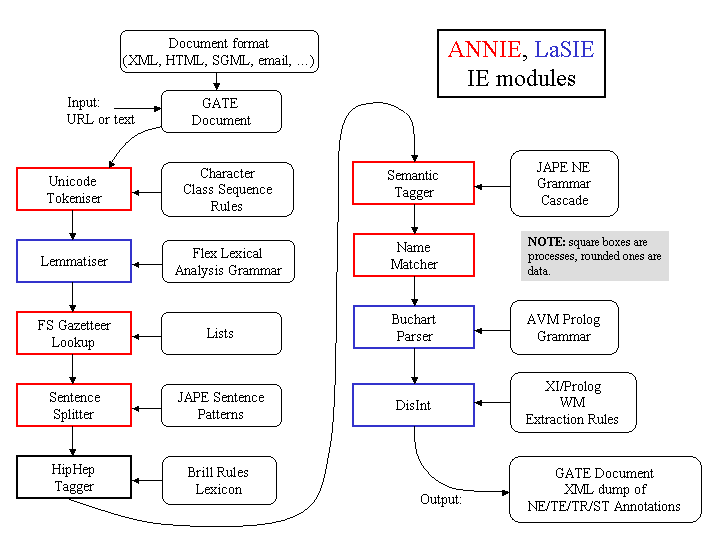
\includegraphics[height=4in]{annie.png}
\end{center}
\caption{ANNIE and LaSIE}
\label{fig:annie1}
\end{figure}
%
ANNIE components are included with GATE (though the linguistic resources they
rely on are generally more simple than the ones we use in-house). The rest of
this \chapthing\ describes these components.

%%%%%%%%%%%%%%%%%%%%%%%%%%%%%%%%%%%%%%%%%%%%%%%%%%%%%%%%%%%%%%%%%%%%%%
\sect[sec:misc-creole:reset]{Document Reset}
%%%%%%%%%%%%%%%%%%%%%%%%%%%%%%%%%%%%%%%%%%%%%%%%%%%%%%%%%%%%%%%%%%%

The document reset resource enables the document to be reset to its
original state, by removing all the annotation sets and their
contents, apart from the one containing the document format analysis
(Original Markups). An optional parameter, keepOriginalMarkupsAS, allows users
to decide whether to keep the Original Markups AS or not while reseting the
document. The parameter \texttt{annotationTypes} can be used to specify
a list of annotation types to remove from all the sets instead of the
whole sets. 

Alternatively, if the parameter \texttt{setsToRemove} is not empty, 
the other parameters except \texttt{annotationTypes}  are ignored 
and only the annotation sets 
specified in this list will be removed. If \texttt{annotationTypes} is also
specified, only those annotation types in the specified sets are removed. 
In order to specify that you want to reset the default
annotation set, just click the "Add" button without entering a name --
this will add \verb|<null>| which denotes the default annotation set.
This resource is normally added to the beginning of an application, so
that a document is reset before an application is rerun on that document.



%%%%%%%%%%%%%%%%%%%%%%%%%%%%%%%%%%%%%%%%%%%%%%%%%%%%%%%%%%%%%%%%%%%%%%%%%%%%%
\sect[sec:annie:tokeniser]{Tokeniser}
%%%%%%%%%%%%%%%%%%%%%%%%%%%%%%%%%%%%%%%%%%%%%%%%%%%%%%%%%%%%%%%%%%%%%%%%%%%%%

The tokeniser splits the text into very simple tokens such as numbers,
punctuation and words of different types. For example, we distinguish
between words in uppercase and lowercase, and between certain types of
punctuation. The aim is to limit the work of the tokeniser to maximise efficiency, and
enable greater flexibility by placing the burden on the grammar rules,
which are more adaptable.

\subsect{Tokeniser Rules}
A rule has a left hand side (LHS) and a right hand side (RHS).
The LHS is a regular expression which has to be matched on the input;
the RHS describes the annotations to be added to the AnnotationSet.
The LHS is separated from the RHS by `$>$'.
The following operators can be used on the LHS:
\begin{small}
\begin{verbatim}
| (or)
* (0 or more occurrences)
? (0 or 1 occurrences)
+ (1 or more occurrences)
\end{verbatim}
\end{small}

\noindent
The RHS uses `;' as a separator, and has the following format:
\begin{small}
\begin{verbatim}
{LHS} > {Annotation type};{attribute1}={value1};...;{attribute
n}={value n}
\end{verbatim}
\end{small}

\noindent
Details about the primitive constructs available are given in the
tokeniser file (DefaultTokeniser.Rules).\\

\noindent
The following tokeniser rule is for a word
beginning with a single capital letter:
\begin{small}
\begin{verbatim}
`UPPERCASE_LETTER' `LOWERCASE_LETTER'* >
  Token;orth=upperInitial;kind=word;
\end{verbatim}
\end{small}
\noindent
It states that the sequence must begin with an uppercase letter,
followed by zero or more lowercase letters. This sequence will then be
annotated as type `Token'. The attribute `orth' (orthography) has
the value `upperInitial'; the attribute `kind' has the value
`word'.

\subsect{Token Types}
In the default set of rules, the following kinds of Token and
SpaceToken are possible:

\subsubsect{Word}
A word is defined as any set of
contiguous upper or lowercase letters, including a hyphen (but no other
forms of punctuation). A word also has the attribute `orth', for which
four values are defined:
\begin{itemize}
\item upperInitial - initial letter is uppercase, rest are lowercase
\item allCaps - all uppercase letters
\item lowerCase - all lowercase letters
\item mixedCaps - any mixture of upper and lowercase letters not
included in the above categories
\end{itemize}

\subsubsect{Number}
A number is defined as any combination of consecutive digits. There
are no subdivisions of numbers.

\subsubsect{Symbol}
Two types of symbol are defined: currency symbol (e.g. `\$', `\pounds') and
symbol (e.g. `\&', `\^{ }').
These are represented by any number of consecutive currency or other
symbols (respectively).

\subsubsect{Punctuation}
Three types of punctuation are defined: start\_punctuation (e.g. `('),
end\_punctuation (e.g. `)'), and other punctuation (e.g. `:'). Each
punctuation symbol is a separate token.


\subsubsect{SpaceToken}
White spaces are divided into two types of SpaceToken - space and
control - according to whether they are pure space characters or
control characters. Any contiguous (and homogeneous) set of space or
control characters is defined as a SpaceToken.

The above description applies to the default tokeniser. However,
alternative tokenisers can be created if necessary. The choice of
tokeniser is then determined at the time of text processing.

%%%%%%%%%%%%%%%%%%%%%%%%%%%%%%%%%%%%%%%%%%%%%%%%%%%%%%%%%%%%%%%%%%%%%%%%%%%%%
\subsect[sec:annie:en-tokeniser]{English Tokeniser}
%%%%%%%%%%%%%%%%%%%%%%%%%%%%%%%%%%%%%%%%%%%%%%%%%%%%%%%%%%%%%%%%%%%%%%%%%%%%%

The English Tokeniser is a processing resource that comprises a normal
tokeniser and a JAPE transducer (see \Chapthing~\ref{chap:jape}). The
transducer has the role of adapting the generic output of the
tokeniser to the requirements of the English part-of-speech
tagger. One such adaptation is the joining together in one token of
constructs like `` '30s'', `` 'Cause'', `` 'em'', `` 'N'', `` 'S'', ``
's'', `` 'T'', `` 'd'', `` 'll'', `` 'm'', `` 're'', `` 'til'', ``
ve'', etc. Another task of the JAPE transducer is to convert negative
constructs like ``don't'' from three tokens (``don'', `` ' `` and
``t'') into two tokens (``do'' and ``n't'').

The English Tokeniser should always be used on English texts that need
to be processed afterwards by the POS Tagger.


%%%%%%%%%%%%%%%%%%%%%%%%%%%%%%%%%%%%%%%%%%%%%%%%%%%%%%%%%%%%%%%%%%%%%%%%%%%%%
\sect[sec:annie:gazetteer]{Gazetteer}
%%%%%%%%%%%%%%%%%%%%%%%%%%%%%%%%%%%%%%%%%%%%%%%%%%%%%%%%%%%%%%%%%%%%%%%%%%%%%

The role of the gazetteer is to identify entity names in the text based on
lists. The ANNIE gazetteer is described here, and also covered in
\Chapthing~\ref{chap:gazetteers} in Section~\ref{sec:gazetteers:anniegaz}.

The gazetteer lists used are plain text files, with one entry per
line. Each list represents a set of names, such as names
of cities, organisations, days of the week, etc.

Below is a small section of the list for units of currency:
\begin{small}
\begin{verbatim}
Ecu
European Currency Units
FFr
Fr
German mark
German marks
New Taiwan dollar
New Taiwan dollars
NT dollar
NT dollars
\end{verbatim}
\end{small}

An index file (lists.def) is used to access these lists; for each list, a
major type is specified and, optionally, a minor type. It is also
possible to include a language in the same way (fourth column), 
where lists for different languages are used, though ANNIE is 
only concerned with monolingual recognition.  By default, the 
Gazetteer PR creates a Lookup annotation for every gazetteer
entry it finds in the text.  One can also specify an annotation type
(fifth column) specific to an individual list.  In the example below, 
the first column refers to the list name, the second column to the
major type, and the third to the minor type.

These lists are compiled into finite state machines. Any text tokens
that are matched by these machines will be annotated with features
specifying the major and minor types. Grammar rules then specify
the types to be identified in particular circumstances. Each 
gazetteer list should reside in the same directory as the index 
file.

\begin{small}
\begin{verbatim}
currency_prefix.lst:currency_unit:pre_amount
currency_unit.lst:currency_unit:post_amount
date.lst:date:specific
day.lst:date:day
\end{verbatim}
\end{small}

So, for example, if a specific day needs to be identified, the minor
type `day' should be specified in the grammar, in order to match 
only information about specific days; if any kind of date needs to be
identified,the major type `date' should be specified, to enable tokens
annotated with any information about dates to be identified. More
information about this can be found in the following section.

In addition, the gazetteer allows arbitrary feature values to be associated
with particular entries in a single list.  ANNIE does not use this capability,
but to enable it for your own gazetteers, set the optional
{\tt gazetteerFeatureSeparator} parameter to a single character (or an escape
sequence such as \verb|\t| or \verb|\uNNNN|) when creating a gazetteer.  In
this mode, each line in a {\tt .lst} file can have feature values specified,
for example, with the following entry in the index file:
\begin{small}\begin{verbatim}
software_company.lst:company:software
\end{verbatim}\end{small}
%
the following \verb|software_company.lst|:
\begin{small}\begin{verbatim}
Red Hat&stockSymbol=RHAT
Apple Computer&abbrev=Apple&stockSymbol=AAPL
Microsoft&abbrev=MS&stockSymbol=MSFT
\end{verbatim}\end{small}
%
and {\tt gazetteerFeatureSeparator} set to \verb|&|, the gazetteer will
annotate \verb|Red Hat| as a \verb|Lookup| with features
\verb|majorType=company|, \verb|minorType=software| and
\verb|stockSymbol=RHAT|.  Note that you do not have to provide the same
features for every line in the file, in particular it is possible to provide
extra features for some lines in the list but not others.

Here is a full list of the parameters used by the Default Gazetteer:

{\bf Init-time parameters}
\begin{description}
\item[listsURL] A URL pointing to the index file (usually lists.def) that 
contains the list of pattern lists. 
\item[encoding] The character encoding to be used while reading the pattern 
lists.
\item[gazetteerFeatureSeparator] The character used to add arbitrary features 
to gazetteer entries. See above for an example.
\item[caseSensitive] Should the gazetteer be case sensitive during matching.
\end{description}

{\bf Run-time parameters}
\begin{description}
\item[document] The document to be processed.
\item[annotationSetName] The name for annotation set where the resulting Lookup 
annotations will be created.
\item[wholeWordsOnly] Should the gazetteer only match whole words? If set to 
true, a string segment in the input document will only be matched if it is 
bordered by characters that are not letters, non spacing marks, or combining 
spacing marks (as identified by the Unicode standard).
\item[longestMatchOnly] Should the gazetteer only match the longest possible
string starting from any position. This parameter is only relevant when the 
list of lookups contains proper prefixes of other entries (e.g when both `Dell'
and `Dell Europe' are in the lists). The default behaviour (when this parameter
is set to {\tt true}) is to only match the longest entry, `Dell Europe' in this 
example. This is the default GATE gazetteer behaviour since version 2.0. Setting
this parameter to {\tt false} will cause the gazetteer to match all possible prefixes.
\end{description}

%%%%%%%%%%%%%%%%%%%%%%%%%%%%%%%%%%%%%%%%%%%%%%%%%%%%%%%%%%%%%%%%%%%%%%%%%%%%%
\sect[sec:annie:splitter]{Sentence Splitter}
%%%%%%%%%%%%%%%%%%%%%%%%%%%%%%%%%%%%%%%%%%%%%%%%%%%%%%%%%%%%%%%%%%%%%%%%%%%%%
The \textbf{sentence splitter} is a cascade of finite-state transducers which
segments the text into sentences. This module is required for the
tagger. The splitter uses a gazetteer list of abbreviations to help
distinguish sentence-marking full stops from other kinds.

Each sentence is annotated with the type `Sentence'.
%% A quoted sentence is also annotated with type Sentence, but has the
%% additional feature `quoted' with value `true'.
Each sentence break (such as a full stop) is also given a `Split'
annotation. It has a feature `kind' with two possible values: `internal' for
any combination of exclamation and question mark or one to four dots and
`external' for a newline.

The sentence splitter is domain and application-independent.

There is an alternative ruleset for the Sentence Splitter which
considers newlines and carriage returns differently. In general this
version should be used when a new line on the page indicates a new
sentence).  To use this alternative version, simply load the
main-single-nl.jape from the default location instead of main.jape
(the default file) when asked to select the location of the grammar
file to be used.


%%%%%%%%%%%%%%%%%%%%%%%%%%%%%%%%%%%%%%%%%%%%%%%%%%%%%%%%%%%%%%%%%%%%%%%%%%%%%
\sect[sec:annie:regex-splitter]{RegEx Sentence Splitter}
%%%%%%%%%%%%%%%%%%%%%%%%%%%%%%%%%%%%%%%%%%%%%%%%%%%%%%%%%%%%%%%%%%%%%%%%%%%%%
The RegEx sentence splitter is an alternative to the standard ANNIE Sentence
Splitter. Its main aim is to address some performance issues identified in the
JAPE-based splitter, mainly do to with improving the execution time and
robustness, especially when faced with irregular input.

As its name suggests, the RegEx splitter is based on regular expressions,
using the default Java implementation.

The new splitter is configured by three files containing (Java style, 
see
\url{http://java.sun.com/j2se/1.5.0/docs/api/java/util/regex/Pattern.html})
regular expressions, one regex per line. The three different files  encode
patterns for:
\begin{description}
  \item[internal splits] sentence splits that are part of the sentence, such
  as sentence ending punctuation;
  \item[external splits] sentence splits that are NOT part of the sentence,
  such as 2 consecutive new lines;
  \item[non splits] text fragments that might be seen as splits but they
  should be ignored (such as full stops occurring inside abbreviations).
\end{description}

The new splitter comes with an initial set of patterns that try to 
emulate the behaviour of the original splitter (apart from the 
situations where the original one was obviously wrong, like not allowing 
sentences to start with a number).

Here is a full list of the parameters used by the RegEx Sentence Splitter:

{\bf Init-time parameters}
\begin{description}
\item[encoding] The character encoding to be used while reading the pattern 
lists.
\item[externalSplitListURL] URL for the file containing the list of external
split patterns;
\item[internalSplitListURL] URL for the file containing the list of internal
split patterns;
\item[nonSplitListURL] URL for the file containing the list of non split
patterns;
\end{description}

{\bf Run-time parameters}
\begin{description}
\item[document] The document to be processed.
\item[outputASName] The name for annotation set where the resulting {\tt
Split} and {\tt Sentence} annotations will be created.
\end{description}

%%%%%%%%%%%%%%%%%%%%%%%%%%%%%%%%%%%%%%%%%%%%%%%%%%%%%%%%%%%%%%%%%%%%%%%%%%%%%
\sect[sec:annie:tagger]{Part of Speech Tagger}
%%%%%%%%%%%%%%%%%%%%%%%%%%%%%%%%%%%%%%%%%%%%%%%%%%%%%%%%%%%%%%%%%%%%%%%%%%%%%
The \textbf{tagger} \cite{Hepple00} is a modified version of the Brill tagger,
which produces a part-of-speech tag as an annotation on each word or symbol.
The list of tags used is given in Appendix \ref{chap:postags}. The tagger uses
a default lexicon and ruleset (the result of training on a large corpus taken
from the Wall Street Journal). Both of these can be modified manually if
necessary. Two additional lexicons exist - one for texts in all uppercase
(lexicon\_cap), and one for texts in all lowercase (lexicon\_lower). To use
these, the default lexicon should be replaced with the appropriate lexicon at
load time. The default ruleset should still be used in this case. 

The ANNIE Part-of-Speech tagger requires the following parameters.
 
\begin{itemize}
\item encoding - encoding to be used for reading rules and lexicons (init-time)
\item lexiconURL - The URL for the lexicon file (init-time)
\item rulesURL - The URL for the ruleset file (init-time)
\item document - The document to be processed (run-time)
\item inputASName - The name of the annotation set used for input (run-time)
\item outputASName - The name of the annotation set used for output (run-time).  This is an optional parameter. If user does not provide any value, new annotations are created under the default annotation set.
\item baseTokenAnnotationType - The name of the annotation type that refers to Tokens in a document (run-time, default = Token)
\item baseSentenceAnnotationType - The name of the annotation type that refers to Sentences in a document (run-time, default = Sentence).
\item outputAnnotationType - POS tags are added as category features on the annotations of type `outputAnnotationType' (run-time, default = Token)
\item posTagAllTokens - If set to false, only Tokens within each baseSentenceAnnotationType will be POS tagged (run-time, default = true).
\item failOnMissingInputAnnotations - if set to false, the PR will not fail with
an ExecutionException if no input Annotations are found and instead only log a 
single warning message per session and a debug message per document that has no
input annotations (run-time, default = true). 
\end{itemize}

If - (inputASName == outputASName) AND (outputAnnotationType ==
baseTokenAnnotationType)

then - 
New features are added on existing annotations of type `baseTokenAnnotationType'.

otherwise - Tagger searches for the annotation of type
`outputAnnotationType' under the `outputASName' annotation set
that has the same offsets as that of the annotation with type
`baseTokenAnnotationType'.  If it succeeds, it adds new feature on a
found annotation, and otherwise, it creates a new annotation of type
`outputAnnotationType' under the `outputASName' annotation set.

%%%%%%%%%%%%%%%%%%%%%%%%%%%%%%%%%%%%%%%%%%%%%%%%%%%%%%%%%%%%%%%%%%%%%%%%%%%%%
\sect[sec:annie:semantic-tagger]{Semantic Tagger}
%%%%%%%%%%%%%%%%%%%%%%%%%%%%%%%%%%%%%%%%%%%%%%%%%%%%%%%%%%%%%%%%%%%%%%%%%%%%%

ANNIE's semantic tagger is based on the JAPE language -- see \Chapthing\
\ref{chap:jape}. It contains rules which act on annotations
assigned in earlier phases, in order to produce outputs of annotated
entities.

The default annotation types, features and possible values produced by ANNIE are based on the original MUC entity types, and are as follows:
\begin{itemize}
\item Person
	\begin{itemize}
	\item gender: male, female
	\end{itemize}
\item Location
	\begin{itemize}
	\item locType: region, airport, city, country, county, province, other
	\end{itemize}
\item Organization
	\begin{itemize}
	\item orgType: company, department, government, newspaper, team, other
	\end{itemize}
\item Money
\item Percent
\item Date
	\begin{itemize}
	\item kind: date, time, dateTime
	\end{itemize}
\item Address
	\begin{itemize}
	\item kind: email, url, phone, postcode, complete, ip, other
	\end{itemize}
\item Identifier
\item Unknown
\end{itemize}

Note that some of these feature values are generated automatically from the gazetteer lists, so if you alter the gazetteer list definition file, these could change. Note also that other annotations, features and values are also created by ANNIE which may be left for debugging purposes: for example, most annotations have a rule feature that gives information about which rule(s) fired to create the annotation.
The Unknown annotation type is used by the Orthomatcher module (see \ref{sec:annie:orthomatcher}) and consists of any proper noun not already identified.



%%%%%%%%%%%%%%%%%%%%%%%%%%%%%%%%%%%%%%%%%%%%%%%%%%%%%%%%%%%%%%%%%%%%%%%%%%%%%
\sect[sec:annie:orthomatcher]{Orthographic Coreference (OrthoMatcher)}
%%%%%%%%%%%%%%%%%%%%%%%%%%%%%%%%%%%%%%%%%%%%%%%%%%%%%%%%%%%%%%%%%%%%%%%%%%%%%

(Note: this component was previously known as a `NameMatcher'.)

% high level description of module's function
The Orthomatcher module adds identity relations between named entities
found by the semantic tagger, in order to perform coreference. It does
not find new named entities as such, but it may assign a type to an
unclassified proper name (an Unknown annotation), using the type of a matching name.

The matching rules are only invoked if the names being compared are
both of the same type, i.e. both already tagged as (say)
organisations, or if one of them is classified as `unknown'.  This
prevents a previously classified name from being recategorised.

\subsect{GATE Interface}

Input -- entity annotations, with an id attribute.

Output -- matches attributes added to the existing entity annotations.

\subsect{Resources}

A lookup table of aliases is used to record non-matching strings which
represent the same entity, e.g. `IBM' and `Big Blue',
`Coca-Cola' and `Coke'. There is also a table of spurious matches,
i.e. matching strings which do not represent the same entity,
e.g. `BT Wireless' and `BT Cellnet' (which are two different
organizations). The list of tables to be used is a load time parameter
of the orthomatcher: a default list is set but can be changed as
necessary.

\subsect{Processing}
%% details of any translations required to produce the required input file

The wrapper builds an array of the strings, types and IDs of all
\texttt{name} annotations, which is then passed to a string comparison
function for pairwise comparisons of all entries.

%For information on how to use the Orthomatcher, see section
%\ref{sec:howto:orthomatcher}.


%%%%%%%%%%%%%%%%%%%%%%%%%%%%%%%%%%%%%%%%%%%%%%%%%%%%%%%%%%%%%%%%%%%%%%%%%%%%%
\sect[sec:annie:pronom-coref]{Pronominal Coreference}
%%%%%%%%%%%%%%%%%%%%%%%%%%%%%%%%%%%%%%%%%%%%%%%%%%%%%%%%%%%%%%%%%%%%%%%%%%%%%
The pronominal coreference module performs anaphora resolution using
the JAPE grammar formalism. Note that this module is not automatically
loaded with the other ANNIE modules, but can be loaded separately as a
Processing Resource. The main module consists of three submodules:
\begin{itemize}
\item quoted text module
\item pleonastic it module
\item pronominal resolution module
\end{itemize}

The first two modules are helper submodules for the pronominal one,
because they do not perform anything related to coreference resolution
except the location of quoted fragments and pleonastic it occurrences
in text.  They generate temporary annotations which are used by the
pronominal submodule (such temporary annotations are removed later).

The main coreference module can operate successfully only if all ANNIE
modules were already executed. The module depends on the following
annotations created from the respective ANNIE modules:

\begin{itemize}
\item Token (English Tokenizer)
\item Sentence (Sentence Splitter)
\item Split (Sentence Splitter)
\item Location (NE Transducer, OrthoMatcher)
\item Person (NE Transducer, OrthoMatcher)
\item Organization (NE Transducer, OrthoMatcher)
\end{itemize}

For each pronoun (anaphor) the coreference module generates an
annotation of type `Coreference' containing two features:

\begin{itemize}

\item antecedent offset - this is the offset of the starting node for
the annotation (entity) which is proposed as the antecedent, or null if no
antecedent can be proposed.

\item matches - this is a list of annotation IDs
that comprise the coreference chain comprising this anaphor/antecedent
pair.

\end{itemize}




\subsect{Quoted Speech Submodule}

The quoted speech submodule identifies quoted fragments in the text
being analysed. The identified fragments are used by the pronominal
coreference submodule for the proper resolution of pronouns such as I,
me, my, etc. which appear in quoted speech fragments.  The module
produces `Quoted Text' annotations.

The submodule itself is a JAPE transducer which loads a JAPE grammar
and builds an FSM over it. The FSM is intended to match the quoted
fragments and generate appropriate annotations that will be used later
by the pronominal module.

The JAPE grammar consists of only four rules, which create temporary
annotations for all punctuation marks that may enclose quoted speech,
such as ", ', `, etc. These rules then try to identify fragments enclosed by
such punctuation. Finally all temporary annotations generated during
the processing, except the ones of type `Quoted Text', are removed
(because no other module will need them later).

\subsect{Pleonastic It Submodule}
The pleonastic it submodule matches pleonastic occurrences of
`it'. Similar to the quoted speech submodule, it is a JAPE
transducer operating with a grammar containing patterns that match the
most commonly observed pleonastic it constructs.


\subsect{Pronominal Resolution Submodule}

The main functionality of the coreference resolution module is in the
pronominal resolution submodule. This uses the result from
the execution of the quoted speech and pleonastic it submodules.
The module works according to the following algorithm:

\begin{itemize}

\item Preprocess the current document. This step locates the
annotations that the submodule need (such as Sentence, Token, Person,
etc.) and prepares the appropriate data structures for them.

\item For each pronoun do the following:
%%
  \begin{itemize}
  \item inspect the proper appropriate context for all candidate
  antecedents for this kind of pronoun;

  \item choose the best antecedent (if any);
  \end{itemize}
%%
\item Create the coreference chains from the individual
  anaphor/antecedent pairs and the coreference information supplied by
  the OrthoMatcher (this step is performed from the main coreference
  module).
\end{itemize}

\subsect{Detailed Description of the Algorithm}

Full details of the pronominal coreference algorithm are as follows.

\subsubsect{Preprocessing}

The preprocessing task includes the following subtasks:

\begin{itemize}
%
\item
%
Identifying the sentences in the document being processed. The
sentences are identified with the help of the Sentence annotations
generated from the Sentence Splitter.  For each sentence a data
structure is prepared that contains three lists. The lists contain the
annotations for the person/organization/location named entities
appearing in the sentence. The named entities in the sentence are
identified with the help of the Person, Location and Organization
annotations that are already generated from the Named Entity
Transducer and the OrthoMatcher.

\item The gender of each person in the sentence is identified and stored in
a global data structure. It is possible that the gender information is
missing for some entities - for example if only the person family name
is observed then the Named Entity transducer will be unable to deduce
the gender. In such cases the list with the matching entities
generated by the OrhtoMatcher is inspected and if some of the
orthographic matches contains gender information it is assigned to the
entity being processed.

\item The identified pleonastic it occurrences are stored in a
separate list. The `Pleonastic It' annotations generated from the
pleonastic submodule are used for the task.


\item For each quoted text fragment, identified by the quoted text
submodule, a special structure is created that contains the persons
and the 3rd person singular pronouns such as `he' and `she' that
appear in the sentence containing the quoted text, but not in the
quoted text span (i.e. the ones preceding and succeeding the quote).

\end{itemize}


\subsubsect{Pronoun Resolution}
This task includes the following subtasks:

Retrieving all the pronouns in the document. Pronouns are represented
as annotations of type `Token' with feature `category' having value
`PRP\$' or `PRP'. The former classifies possessive adjectives such as
my, your, etc.  and the latter classifies personal, reflexive
etc. pronouns. The two types of pronouns are combined in one list and
sorted according to their offset in the text.


For each pronoun in the list the following actions are performed:
  \begin{itemize}
  %
  \item
  If the pronoun is `it', then the module performs a check to determine if this is a
  pleonastic occurrence.  If it is, then no further attempt for
  resolution is made.

  \item
  The proper context is determined. The context size is expressed in
  the number of sentences it will contain. The context always includes
  the current sentence (the one containing the pronoun), the preceding
  sentence and zero or more preceding sentences.

  \item
  Depending on the type of pronoun, a set of candidate antecedents is
  proposed. The candidate set includes the named entities that are
  compatible with this pronoun. For example if the current pronoun is
  she then only the Person annotations with `gender' feature equal to
  `female' or `unknown' will be considered as candidates.

  \item
  From all candidates, one is chosen according to evaluation criteria
  specific for the pronoun.
  \end{itemize}


\subsubsect{Coreference Chain Generation}

This step is actually performed by the
main module. After executing each of the submodules on the current
document, the coreference module follows the steps:

  \begin{itemize}
  \item
  Retrieves the anaphor/antecedent pairs generated from them.

  \item
  For each pair, the orthographic matches (if any) of the antecedent
  entity is retrieved and then extended with the anaphor of the pair
  (i.e. the pronoun). The result is the coreference chain for the
  entity. The coreference chain contains the IDs of the annotations
  (entities) that co-refer.

  \item
  A new Coreference annotation is created for each chain. The
  annotation contains a single feature `matches' whose value is the
  coreference chain (the list with IDs). The annotations are exported
  in a pre-specified annotation set.
  \end{itemize}
%


The resolution of she, her, her\$, he, him, his, herself and himself
are similar because an analysis of a corpus showed that these
pronouns are related to their antecedents in a similar manner. The
characteristics of the resolution process are:

  \begin{itemize}
  \item
  Context inspected is not very big - cases where the antecedent is
  found more than 3 sentences back from the anaphor are rare.

  \item
  Recency factor is heavily used - the candidate antecedents that
  appear closer to the anaphor in the text are scored better.

  \item
  Anaphora have higher priority than cataphora. If there is an
  anaphoric candidate and a cataphoric one, then the anaphoric one is
  preferred, even if the recency factor scores the cataphoric
  candidate better.
  \end{itemize}

The resolution process performs the following steps:
  \begin{itemize}

  \item
  Inspect the context of the anaphor for candidate antecedents. Every
  Person annotation is consider to be a candidate. Cases where she/her
  refers to inanimate entity (ship for example) are not handled.

  \item
  For each candidate perform a gender compatibility check - only
  candidates having `gender' feature equal to `unknown' or compatible
  with the pronoun are considered for further evaluation.

  \item
  Evaluate each candidate with the best candidate so far. If the two
  candidates are anaphoric for the pronoun then choose the one that
  appears closer. The same holds for the case where the two candidates
  are cataphoric relative to the pronoun. If one is anaphoric and the
  other is cataphoric then choose the former, even if the latter
  appears closer to the pronoun.

  \end{itemize}


\subsubsect{Resolution of `it', `its', `itself'}

This set of pronouns also shares many common characteristics. The
resolution process contains certain differences with the one for the
previous set of pronouns. Successful resolution for it, its, itself is
more difficult because of the following factors:

  \begin{itemize}
  \item
  There is no gender compatibility restriction. In the case in which there
  are several candidates in the context, the gender compatibility
  restriction is very useful for rejecting some of the
  candidates. When no such restriction exists, and with the lack of
  any syntactic or ontological information about the entities in the
  context, the recency factor plays the major role in choosing the
  best antecedent.

  \item
  The number of nominal antecedents (i.e. entities that are not referred
  by name) is much higher compared to the number of such
  antecedents for she, he, etc. In this case trying to find an antecedent
  only amongst named entities degrades the precision a lot.
  \end{itemize}

%%
\subsubsect{Resolution of `I', `me', `my', `myself'}

Resolution of these pronouns is dependent on the work of the quoted speech submodule.
One important difference from the resolution process of other pronouns
is that the context is not measured in sentences but depends solely on
the quote span. Another difference is that the context is not
contiguous - the quoted fragment itself is excluded from the context,
because it is unlikely that an antecedent for I, me, etc. appears
there. The context itself consists of:
  \begin{itemize}
  \item
  the part of the sentence where the quoted fragment originates, that
is not contained in the quote - i.e. the text prior to the quote;

  \item
  the part of the sentence where the quoted fragment ends, that is not
  contained in the quote - i.e. the text following the quote;

  \item
  the part of the sentence preceding the sentence where the quote
  originates, which is not included in other quote.
  \end{itemize}

It is worth noting that contrary to other pronouns, the antecedent for
I, me, my and  myself is most often cataphoric or if anaphoric it is
not in the same sentence with the quoted fragment.

The resolution algorithm consists of the following steps:
  \begin{itemize}
  \item
  Locate the quoted fragment description that contains the pronoun. If
  the pronoun is not contained in any fragment then return without
  proposing an antecedent.

  \item
  Inspect the context for the quoted fragment (as defined above) for
  candidate antecedents. Candidates are considered annotations of type
  Pronoun or annotations of type Token with features {category =
  `PRP', string = `she'} or {category = `PRP', string = `he'}.

  \item
  Try to locate a candidate in the text succeeding the quoted fragment
  (first pattern). If more than one candidate is present, choose the
  closest to the end of the quote. If a candidate is found then
  propose it as antecedent and exit.

  \item
  Try to locate a candidate in the text preceding the quoted fragment
  (third pattern). Choose the closest one to the beginning of the
  quote. If found then set as antecedent and exit.

  \item
  Try to locate antecedents in the unquoted part of the sentence
  preceding the sentence where the quote starts (second pattern). Give
  preference to the one closest to the end of the quote (if any) in
  the preceding sentence or closest to the sentence beginning.
  \end{itemize}



%%%%%%%%%%%%%%%%%%%%%%%%%%%%%%%%%%%%%%%%%%%%%%%%%%%%%%%%%%%%%%%%%%%%%%%%%%%%%
\sect[sec:annie:annie-example]{A Walk-Through Example}
%%%%%%%%%%%%%%%%%%%%%%%%%%%%%%%%%%%%%%%%%%%%%%%%%%%%%%%%%%%%%%%%%%%%%%%%%%%%%

Let us take an example of a 3-stage procedure using the tokeniser, gazetteer
and named-entity grammar. Suppose we wish to recognise the phrase
`800,000 US dollars' as an entity of type `Number', with the
feature `money'.

First of all, we give an example of a grammar rule (and corresponding
macros) for money, which would recognise this type of pattern.

\begin{small}
\begin{verbatim}
Macro: MILLION_BILLION
({Token.string == "m"}|
{Token.string == "million"}|
{Token.string == "b"}|
{Token.string == "billion"}
)

Macro: AMOUNT_NUMBER
({Token.kind == number}
(({Token.string == ","}|
  {Token.string == "."})
{Token.kind == number})*
(({SpaceToken.kind == space})?
 (MILLION_BILLION)?)
)

Rule:	Money1
// e.g. 30 pounds
  (
      (AMOUNT_NUMBER)
      (SpaceToken.kind == space)?
      ({Lookup.majorType == currency_unit})
  )
 :money  -->
  :money.Number = {kind = "money", rule = "Money1"}
\end{verbatim}
\end{small}


\subsect{Step 1 - Tokenisation}

The tokeniser separates this phrase into the following tokens. In
general, a word is comprised of any number of letters of either case, including a
hyphen, but nothing else; a number is composed of any sequence of
digits; punctuation is recognised individually (each character is a
separate token), and any number of consecutive spaces
and/or control characters are recognised as a single spacetoken.

\begin{small}
\begin{verbatim}
Token, string = `800', kind = number, length = 3
Token, string = `,', kind = punctuation, length = 1
Token, string = `000', kind = number, length = 3
SpaceToken, string = ` ', kind = space, length = 1
Token, string = `US', kind = word, length = 2, orth = allCaps
SpaceToken, string = ` ', kind = space, length = 1
Token, string = `dollars', kind = word, length = 7, orth = lowercase
\end{verbatim}
\end{small}

\subsect{Step 2 - List Lookup}

The gazetteer lists are then searched to find all occurrences of
matching words in the text. It finds the following match for the
string `US dollars':

\begin{small}
\begin{verbatim}
Lookup, minorType = post_amount, majorType = currency_unit
\end{verbatim}
\end{small}

\subsect{Step 3 - Grammar Rules}

The grammar rule for money is then invoked.
The macro MILLION\_BILLION recognises any of the strings `m',
`million', `b', `billion'. Since none of these exist in the
text, it passes onto the next macro. The AMOUNT\_NUMBER macro
recognises a number, optionally followed by any number of sequences of
the form`dot or comma plus number', followed by an optional space
and an optional MILLION\_BILLION. In this case, `800,000' will be
recognised. Finally, the rule Money1 is invoked. This recognises the
string identified by the AMOUNT\_NUMBER macro, followed by an optional
space, followed by a unit of currency (as determined by the
gazetteer). In this case, `US dollars' has been identified as a
currency unit, so the rule Money1 recognises
the entire string `800,000 US dollars'. Following the rule, it will
be annotated as a Number entity of type Money:

\begin{small}\begin{verbatim} Number, kind = money, rule = Money1 \end{verbatim}\end{small}










